\documentclass[UTF8]{ctexart}
\usepackage{cite}
\usepackage{geometry}
\usepackage{indentfirst}
\usepackage{hyperref}
\usepackage{harpoon}
\usepackage{amsmath}
\usepackage{amssymb}
\usepackage{graphicx}
\usepackage{float}
\usepackage{subfigure}
\usepackage{multirow}
\usepackage{array}
\usepackage{relsize}
\usepackage{tikz}
\usetikzlibrary{arrows, shapes, positioning, calc}
\geometry{a4paper, left=1cm, right=1cm, top=2cm, bottom=2cm}
\setlength{\parindent}{1cm}
\renewcommand\contentsname{Content}
\newcommand{\lint}{\mathlarger{\int}}
\title{正交多项式}
\author{段元兴}
\date{\today}
\begin{document}
\maketitle
\thispagestyle{empty}
\setcounter{page}{1}
\newpage
\tableofcontents
\newpage
    \section{}
        \subsection{}
            \indent 证明: 当$i=j$时
            \begin{equation}
                \left<Q_i|Q_j\right>=\dfrac{\left<V_i|V_i\right>}{\alpha_i^2}=1=\delta_{ij}
            \end{equation}
            当$i>j$时, 假设$\left<Q_{i-1}|Q_j\right>=0$成立($i-1\neq j$), 现证明$\left<Q_i|Q_j\right>=0$:
            \begin{equation}
                \begin{array}{ll}
                \left<Q_i|Q_j\right>&=\dfrac{\left<xQ_{i-1}-\sum\limits_{k=0}^{i-1}\left<Q_k|xQ_{i-1}\right>Q_k\bigg{|}Q_j\right>}{\alpha_i\alpha_j}\\
                &=\dfrac{\left<xQ_{i-1}|Q_j\right>-\sum\limits_{k=0}^{i-1}\left<Q_k|xQ_{i-1}\right>\left<Q_k|Q_j\right>}{\alpha_i\alpha_j}\\
                &=\dfrac{\left<xQ_{i-1}|Q_j\right>-\left<Q_{j}|xQ_{i-1}\right>\left<Q_j|Q_j\right>}{\alpha_i\alpha_j}\\
                &=0\\
                \end{array}
            \end{equation}
        \subsection{}
            \indent 证明: 对于$i=0,1,\dots,n-3$:
            \begin{equation}
                \begin{array}{ll}
                    \gamma_{i,n-1}&=\left<Q_i|xQ_{n-1}\right>\\
                    &=\left<\alpha_{i+1}Q_{i+1}+\sum\limits_{k=0}^i\left<Q_k|xQ_i\right>Q_k\bigg{|}Q_{n-1}\right>\\
                    &=\alpha_{i+1}\left<Q_{i+1}|Q_{n-1}\right>+\sum\limits_{k=0}^i\left<Q_k|xQ_i\right>\left<Q_k|Q_{n-1}\right>\\
                    &=0\\
                \end{array}
            \end{equation}
        \subsection{}
            \indent 证明: 由1.2可知:
            \begin{equation}
                \begin{array}{ll}
                \gamma_{n-1, n}&=\alpha\left<Q_n|Q_n\right>+\sum\limits_{k=0}^n-1\left<Q_k|xQ_i\right>\left<Q_k|Q_n\right>\\
                &=\alpha
                \end{array}
            \end{equation}
    \section{}
        \subsection{}
            \indent 由于给出的Legendre多项式递推公式是对已经归一化的, 为减小计算根号的误差, 可以利用未归一化的公式:
            \begin{equation}
                (2*n+1)xV_n(x)=nV_{n-1}(x)+(n+1)V_{n+1}(x)
            \end{equation}
            其中
            \begin{equation}
                V_n(x)=\sqrt{\dfrac{2}{2n+1}}P_n(x)
            \end{equation}
            且$V_0(x)=1,V_1(x)=x$.\\
            \indent 计算结果如下表:
            \begin{table}[H]
                \centering
                \caption{}
                \begin{tabular}{|c|c|c|}
                    \hline
                    &Legendre&Laguerre\\
                    \hline
                    2&-0.1976423538&0.1250000000\\
                    \hline
                    16&-0.6087144379&0.09265564419\\
                    \hline
                    128&-0.2214407353&-0.2278406909\\
                    \hline
                    1024&-0.6063038195&0.1340328657\\
                    \hline
                \end{tabular}
            \end{table}
        \subsection{}
            \indent 由Hermite多项式的递推公式知:
            \begin{equation}
                \alpha_i=\sqrt{\dfrac{i+1}{2}},\beta_i=0,i=0,1,\dots
            \end{equation}
            而对于Chebyshev多项式有
            \begin{equation}
                \alpha_0=\dfrac{1}{\sqrt{2}},\alpha_i=\dfrac{1}{2},i=1,2,\dots,\beta_i=0,i=0,1,\dots
            \end{equation}
            写到对称三对角矩阵后即可使用带位移的隐式对称QR求本征值. 以下是计算结果和耗时:
            \begin{table}[H]
                \centering
                \caption{求解Hermite多项式和Chebyshev多项式的根耗时(CPU: Ryzen9 3950x, 单线程, 仅含求解特征值的时间, 单位: ms)}
                \begin{tabular}{|c|c|c|c|}
                    \hline
                    规模&Hermite多项式&Chebyshev多项式&Chebyshev多项式根的正确性 (所有根的误差均小于$10^{-14}$)\\
                    \hline
                    2&0.002&0.000&是\\
                    \hline
                    16&0.011&0.011&是\\
                    \hline
                    128&0.515&0.507&是\\
                    \hline
                    1024&28.068&28.118&是\\
                    \hline
                \end{tabular}
            \end{table}
        \subsection{}
            \indent 证明: 由对应不同特征值的特征向量的正交性和零点得:
            \begin{equation}
                \begin{array}{ll}
                    f_j(x_i)&=\sum\limits_{k=0}^{n-1}Q_k(x_i)Q_k(x_j)\\
                    &=
                    \left\{
                    \begin{array}{cc}
                        0,&i\neq j\\
                        \sum\limits_{k=0}^{n-1}Q_k(x_i)Q_k(x_i)=\dfrac{1}{\omega_i^2},&i=j\\
                    \end{array}
                    \right..
                \end{array}
            \end{equation}
            即证明其是在高斯节点上的插值多项式. 现证明对于任何不超过$2n-1$次的多项式$f(x)$均有
            \begin{equation}
                \lint_a^bf(x)\rho(x)dx=\lint_a^b\sum\limits_{k=0}^{n-1}f(x_k)g_k(x)\rho(x)dx=\sum\limits_{k=0}^{n-1}f(x_k)A_k.
            \end{equation}
            其中
            \begin{equation}
                A_k=\lint_a^bg_k(x)\rho(x)dx,
            \end{equation}
            而
            \begin{equation}
                g_k(x)=\omega_k^2f_k(x)
            \end{equation}
            为归一化后的基函数. 设$\Omega_n(x)=\prod\limits_{k=0}^{n-1}(x-x_i)$, 通过多项式除法得到:
            \begin{equation}
                f(x)=\Omega_n(x)q(x)+r(x).
            \end{equation}
            其中$q(x), r(x)$均为不超过$n-1$次的多项式. 从而
            \begin{equation}
                \lint_a^bf(x)dx=\lint_a^b\Omega_n(x)\rho(x)q(x)dx+\lint_a^br(x)\rho(x)dx
            \end{equation}
            由于对于不超过$n-1$次的多项式, 其插值得到的积分式精确的, 所以对$r(x)$的积分是精确的. 而
            由于$\Omega_n(x)$与$Q_n(x)$的次数和零点一致, 所以仅差一个常数系数, 又任意小于等于$n-1$次
            的多项式可以用$\{Q_0(x),Q_1(x),\dots,Q_{n-1}(x)\}$展开, 故
            \begin{equation}
                \lint_a^b\Omega_n(x)\rho(x)q(x)dx=0
            \end{equation}
            得证.\\
            \indent 现求其系数: 从上面的证明可以看出权值
            \begin{equation}
                \begin{array}{ll}
                    A_j&=\lint_a^bg_j(x)\rho(x)dx\\
                    &=\sum\limits_{i=0}^{n-1}\lint_a^b\omega_j^2Q_i(x_j)Q_i(x)\rho(x)dx\\
                    &=\sum\limits_{i=0}^{n-1}\omega_j^2\left<Q_0|Q_0\right>=\omega_j^2.
                \end{array}
            \end{equation}
            下表是求出不同规模的$A_j$的耗时 (1024阶Hermite多项式在计算时超出了double的范围):
            \begin{table}[H]
                \centering
                \caption{求基函数权重$A_j$的耗时(CPU: Ryzen9 3950x, 单线程, 单位: ms)}
                \begin{tabular}{|c|c|c|}
                    \hline
                    耗时&Hermite多项式&Chebyshev多项式\\
                    \hline
                    2&0.005&0.000\\
                    \hline
                    16&0.022&0.003\\
                    \hline
                    128&10.263&1.196\\
                    \hline
                    1024&-&736.279\\
                    \hline
                \end{tabular}
            \end{table}
            \indent 对于$N=2, 16, 128$, 分别做出$j=0,\dfrac{N}{2}$的各种图像:
            \begin{figure}[H]
                \centering
                \subfigure[Hermite(2), $j=0,1$]{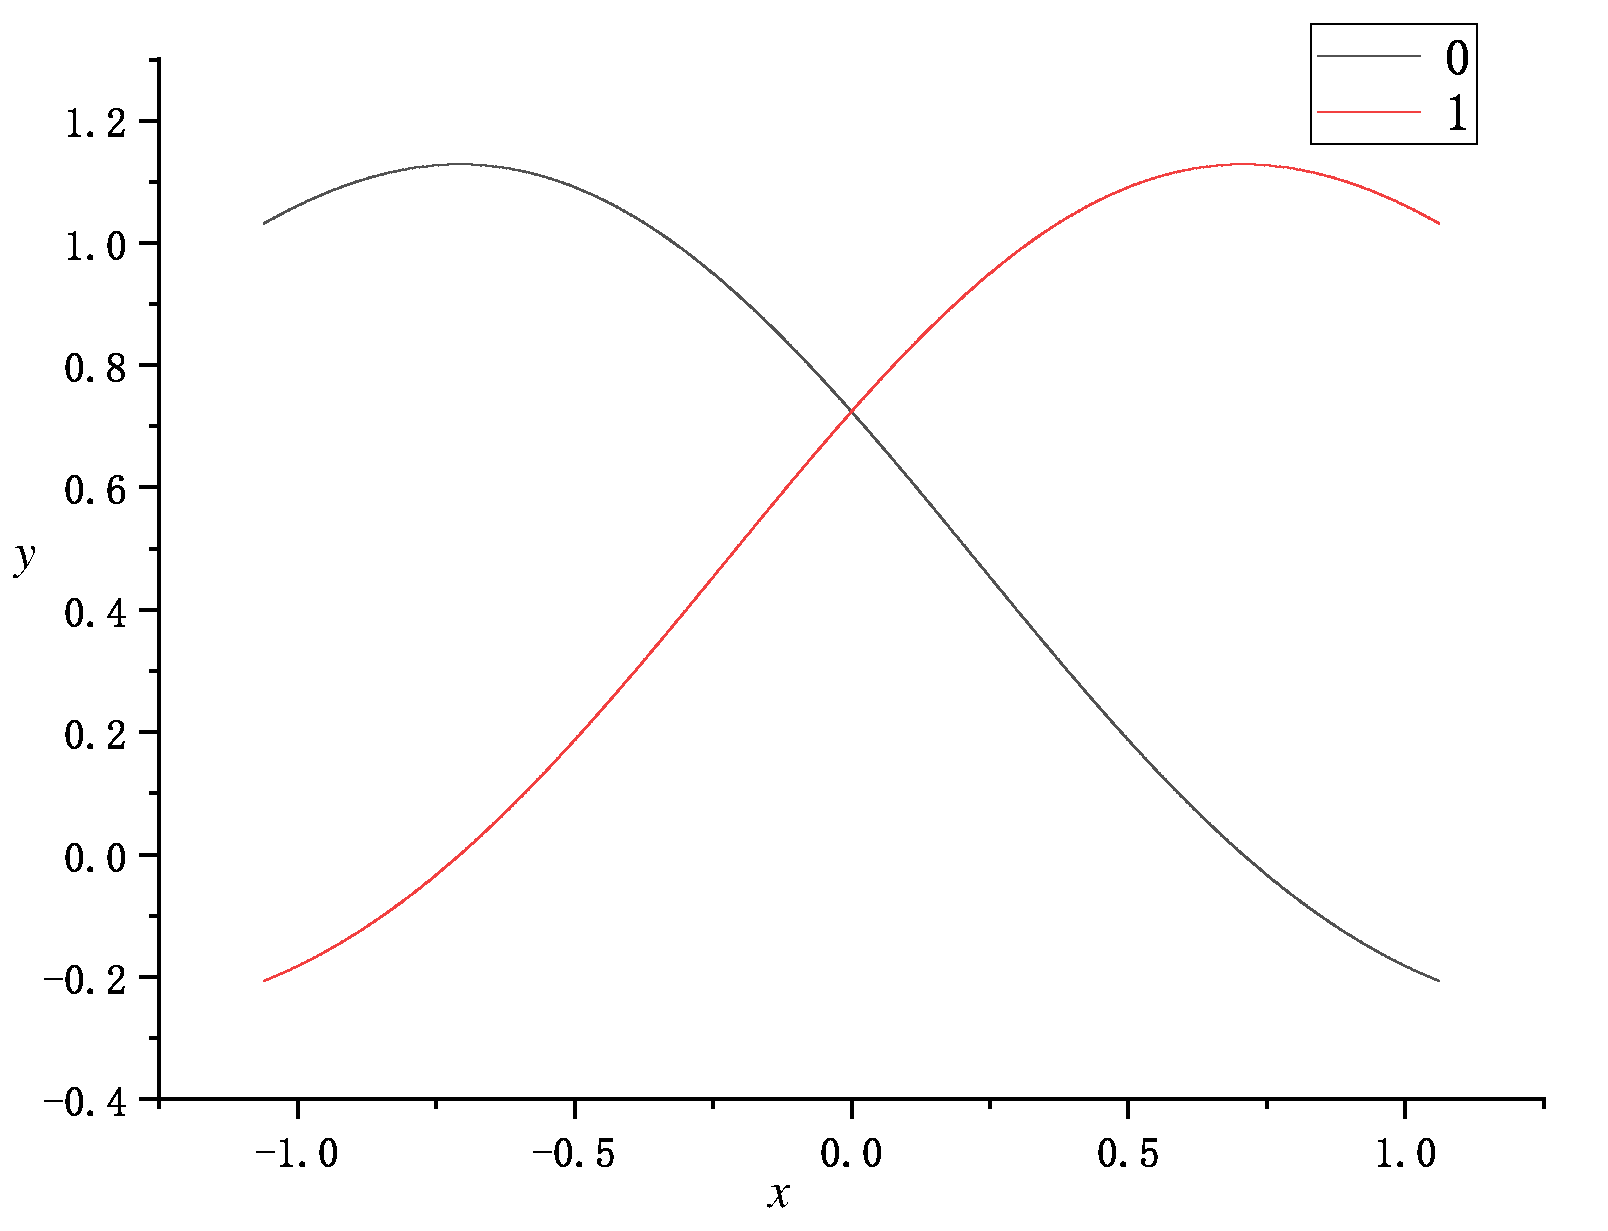
\includegraphics[width=5.5cm]{1.pdf}}\quad
                \subfigure[Hermite(16), $j=0$]{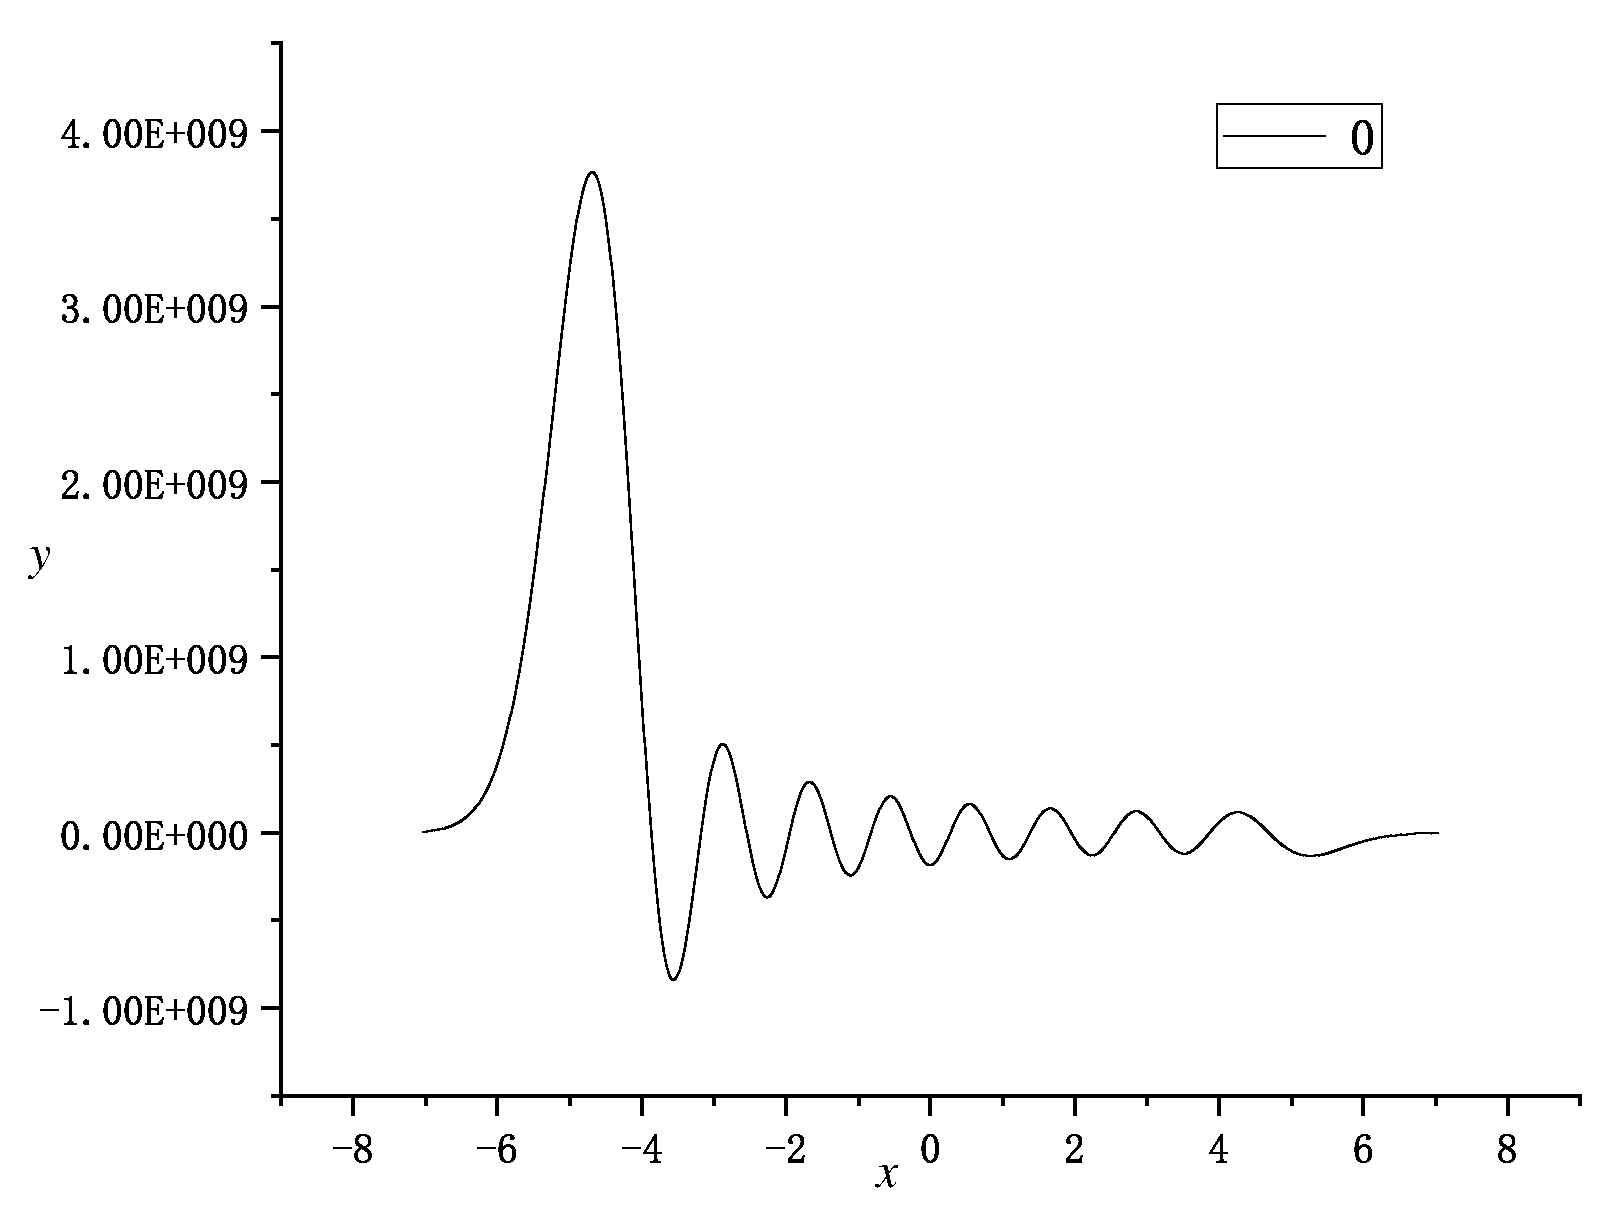
\includegraphics[width=5.5cm]{2.pdf}}\quad
                \subfigure[Hermite(16), $j=8$]{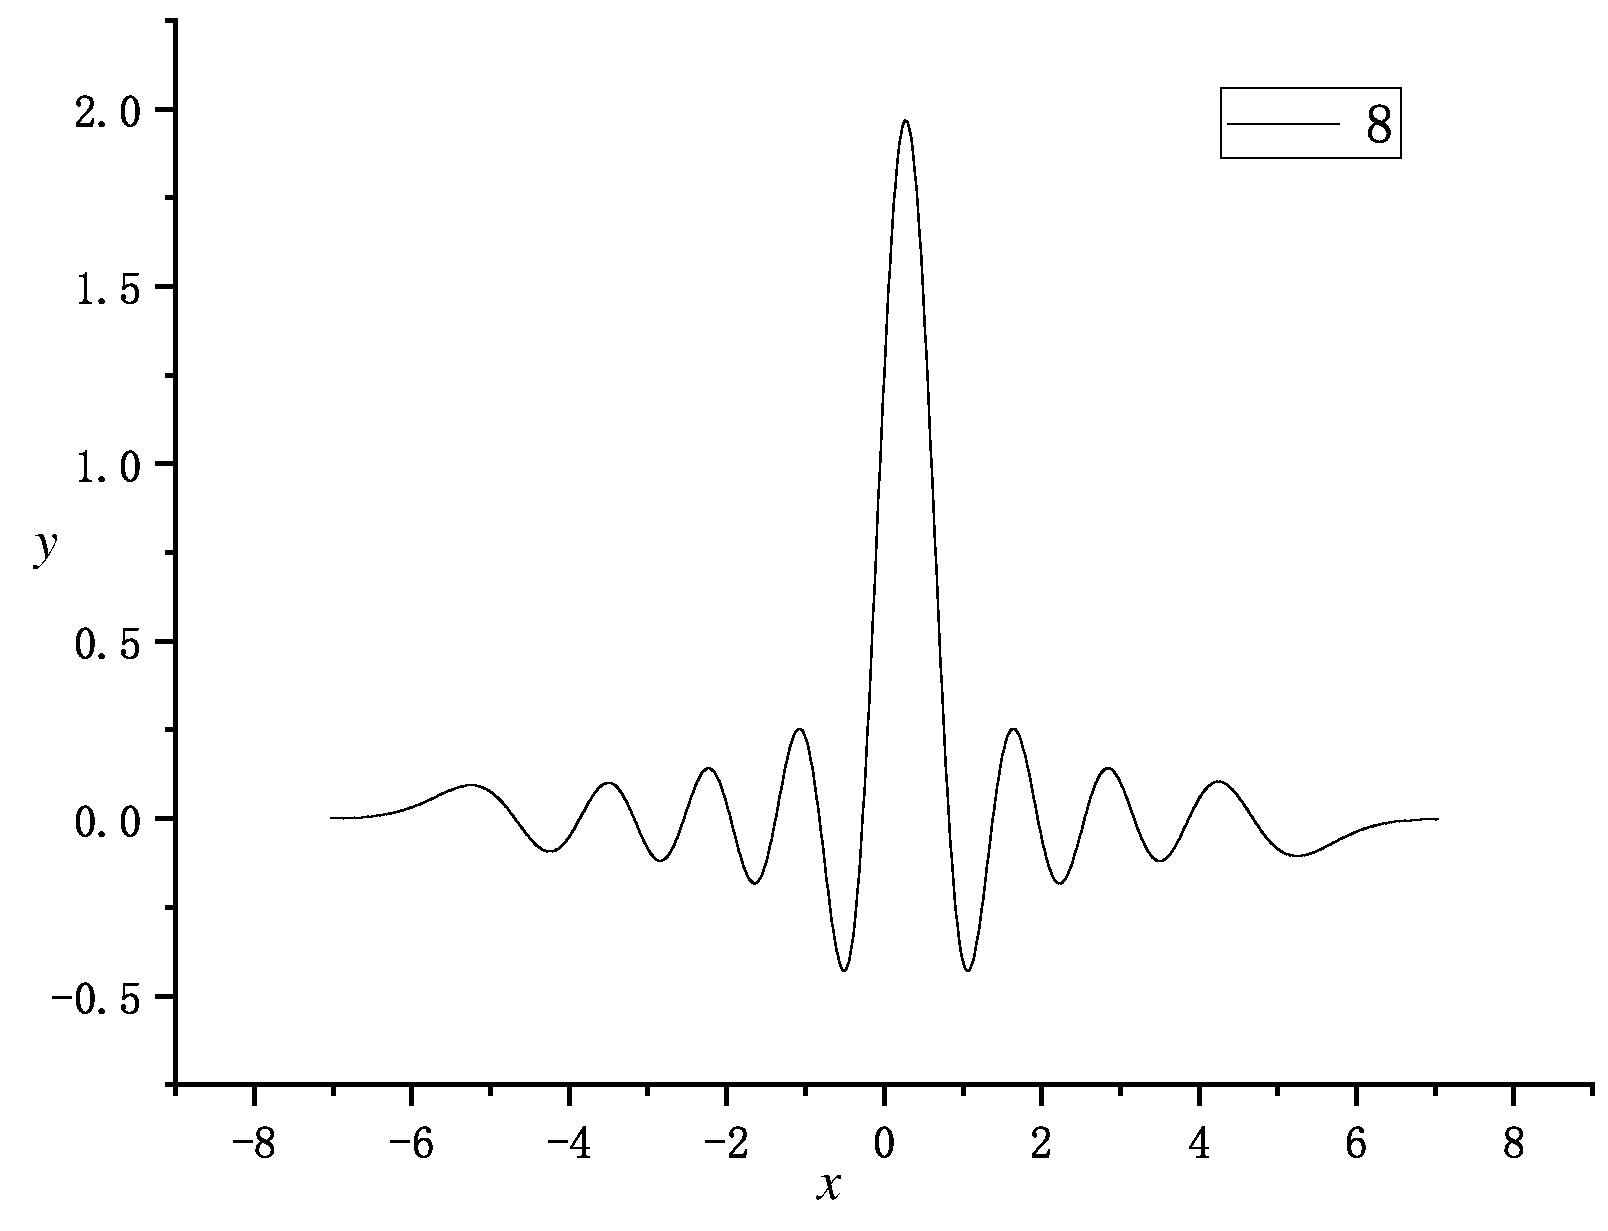
\includegraphics[width=5.5cm]{3.pdf}}\quad
                \subfigure[Hermite(128), $j=0$]{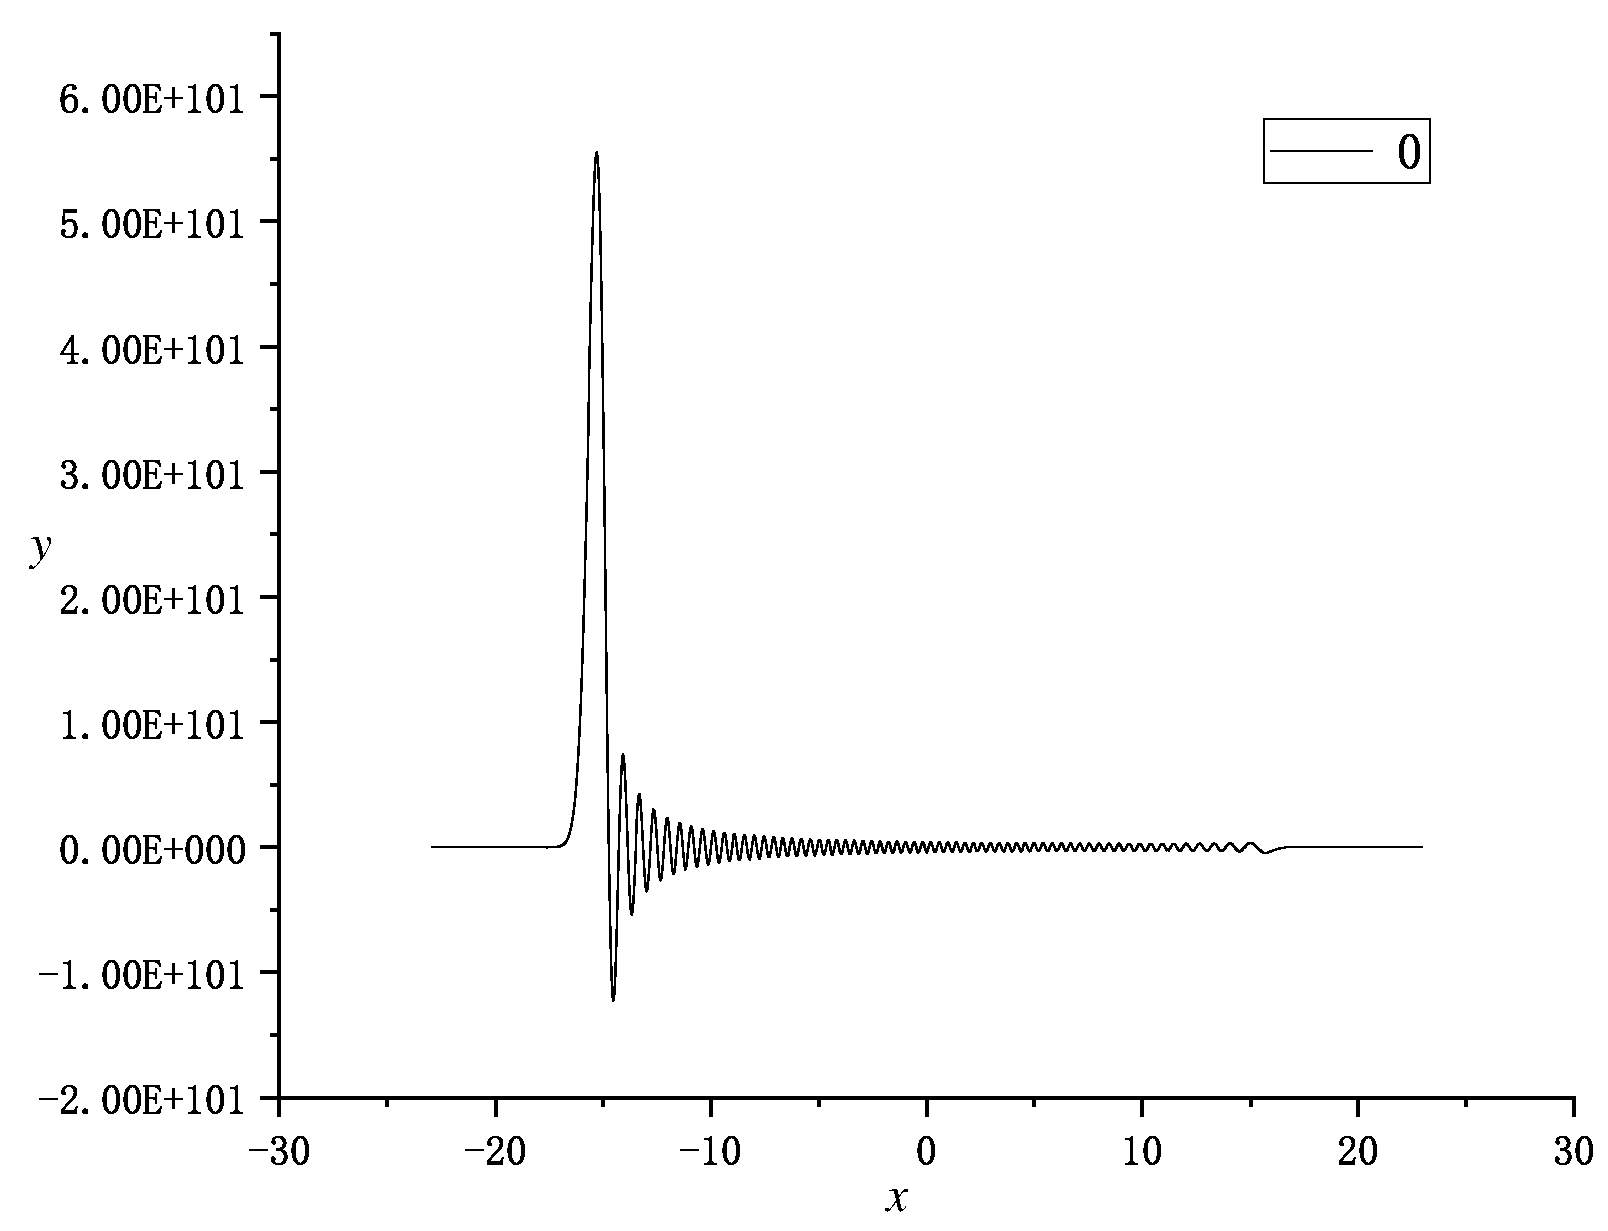
\includegraphics[width=5.5cm]{4.pdf}}\quad
                \subfigure[Hermite(128), $j=64$]{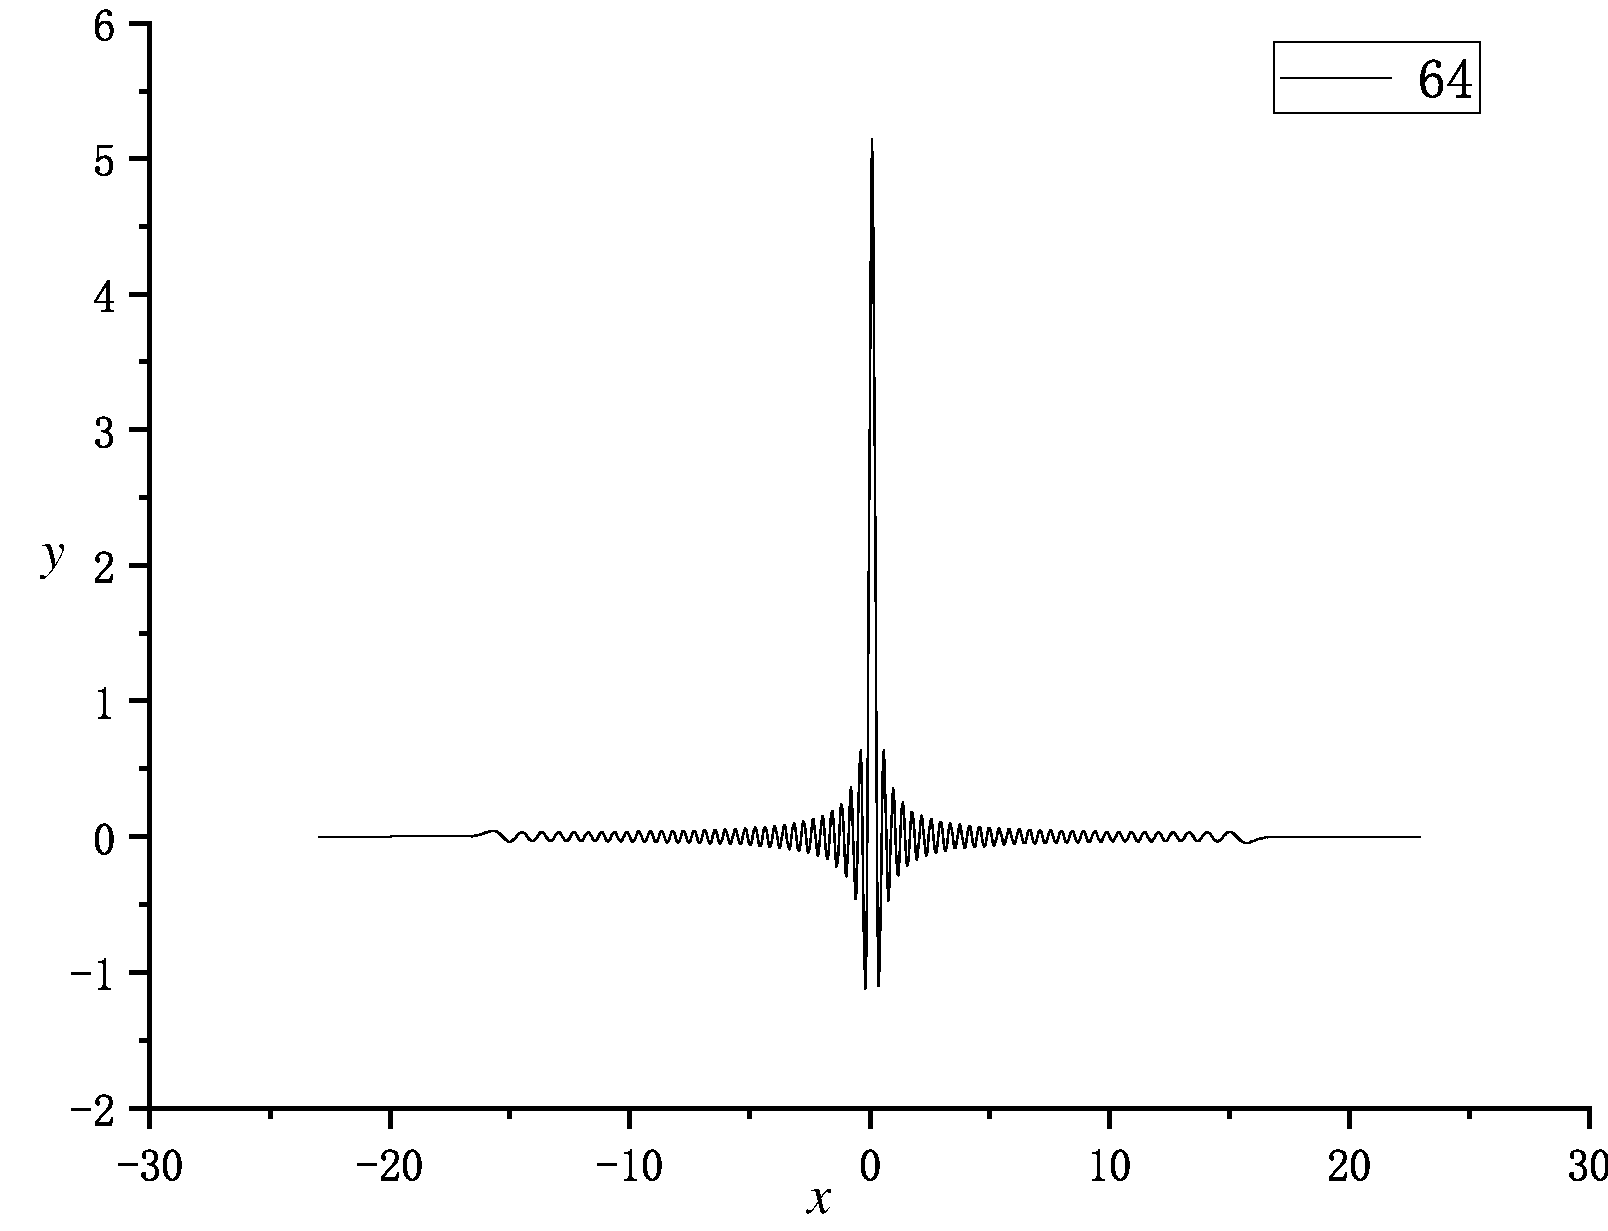
\includegraphics[width=5.5cm]{5.pdf}}\quad
                \subfigure[Chebyshev(2), $j=0,1$]{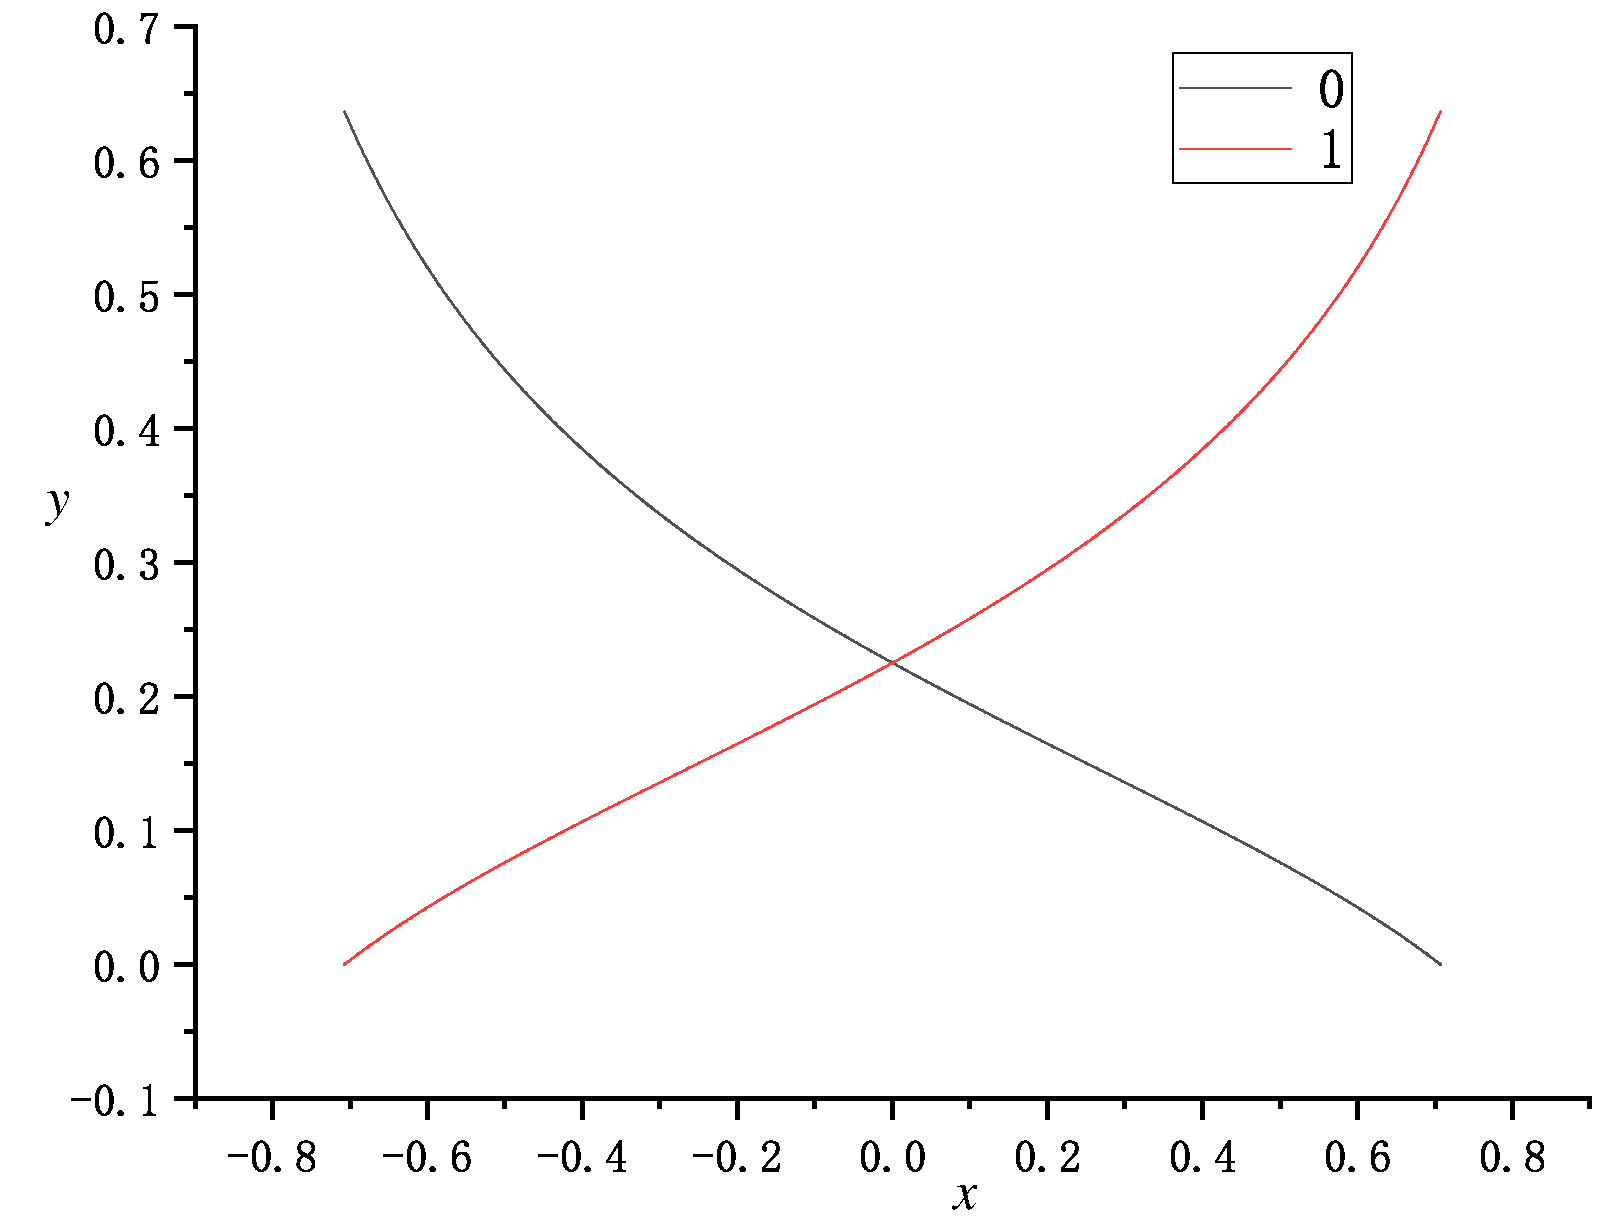
\includegraphics[width=5.5cm]{6.pdf}}\quad
                \subfigure[Chebyshev(16), $j=0$]{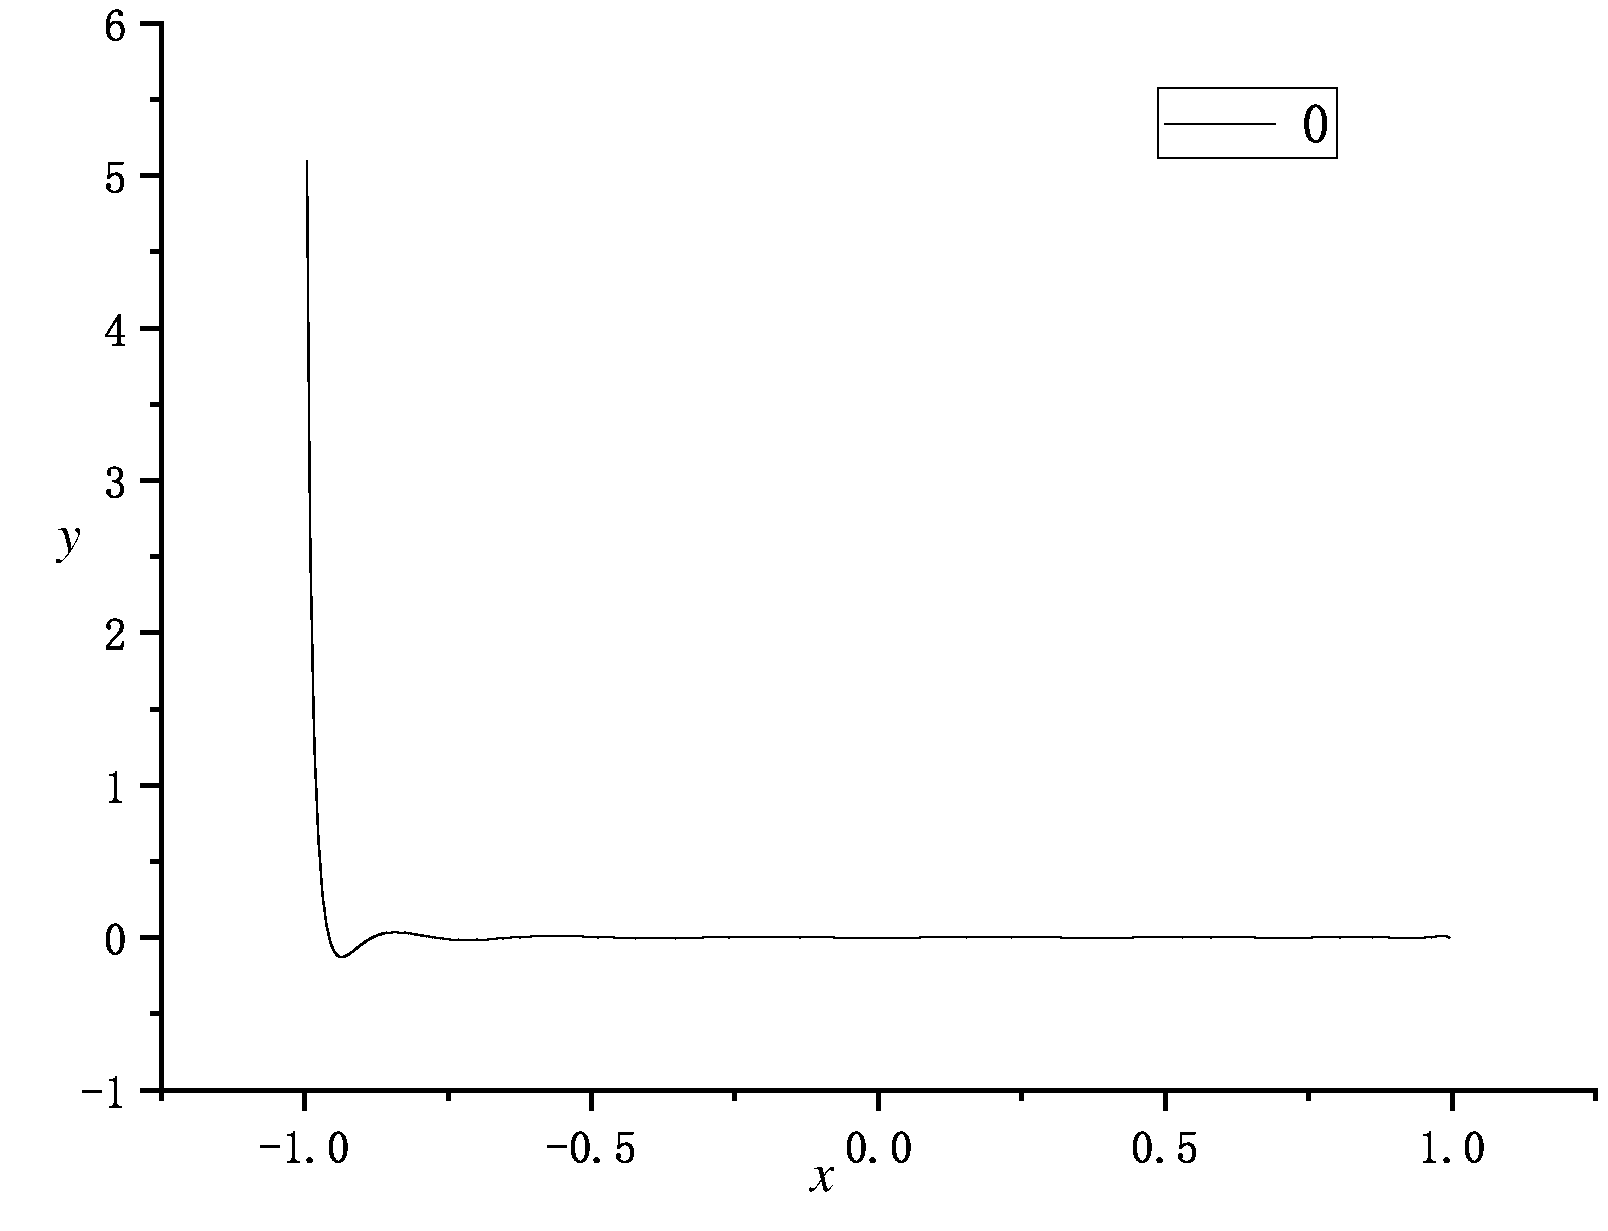
\includegraphics[width=5.5cm]{7.pdf}}\quad
                \subfigure[Chebyshev(16), $j=0,8$]{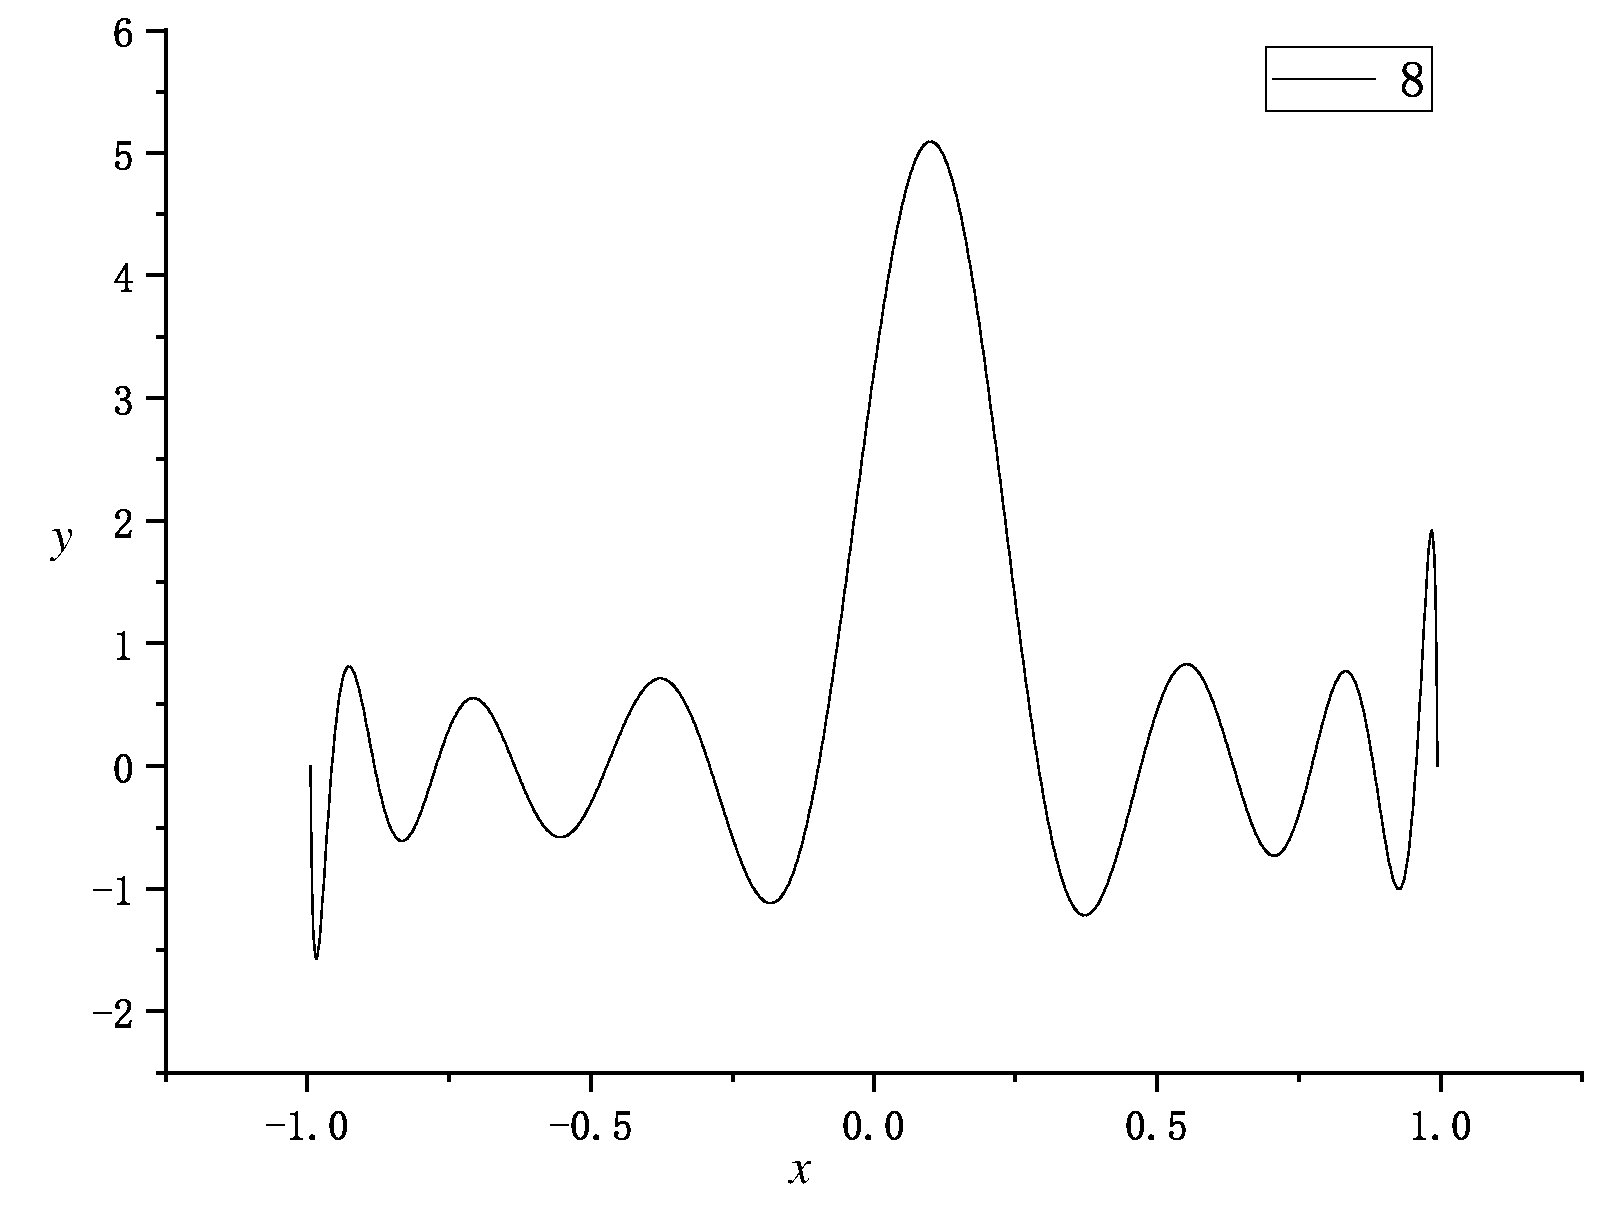
\includegraphics[width=5.5cm]{8.pdf}}\quad
                \subfigure[Chebyshev(128), $j=0$]{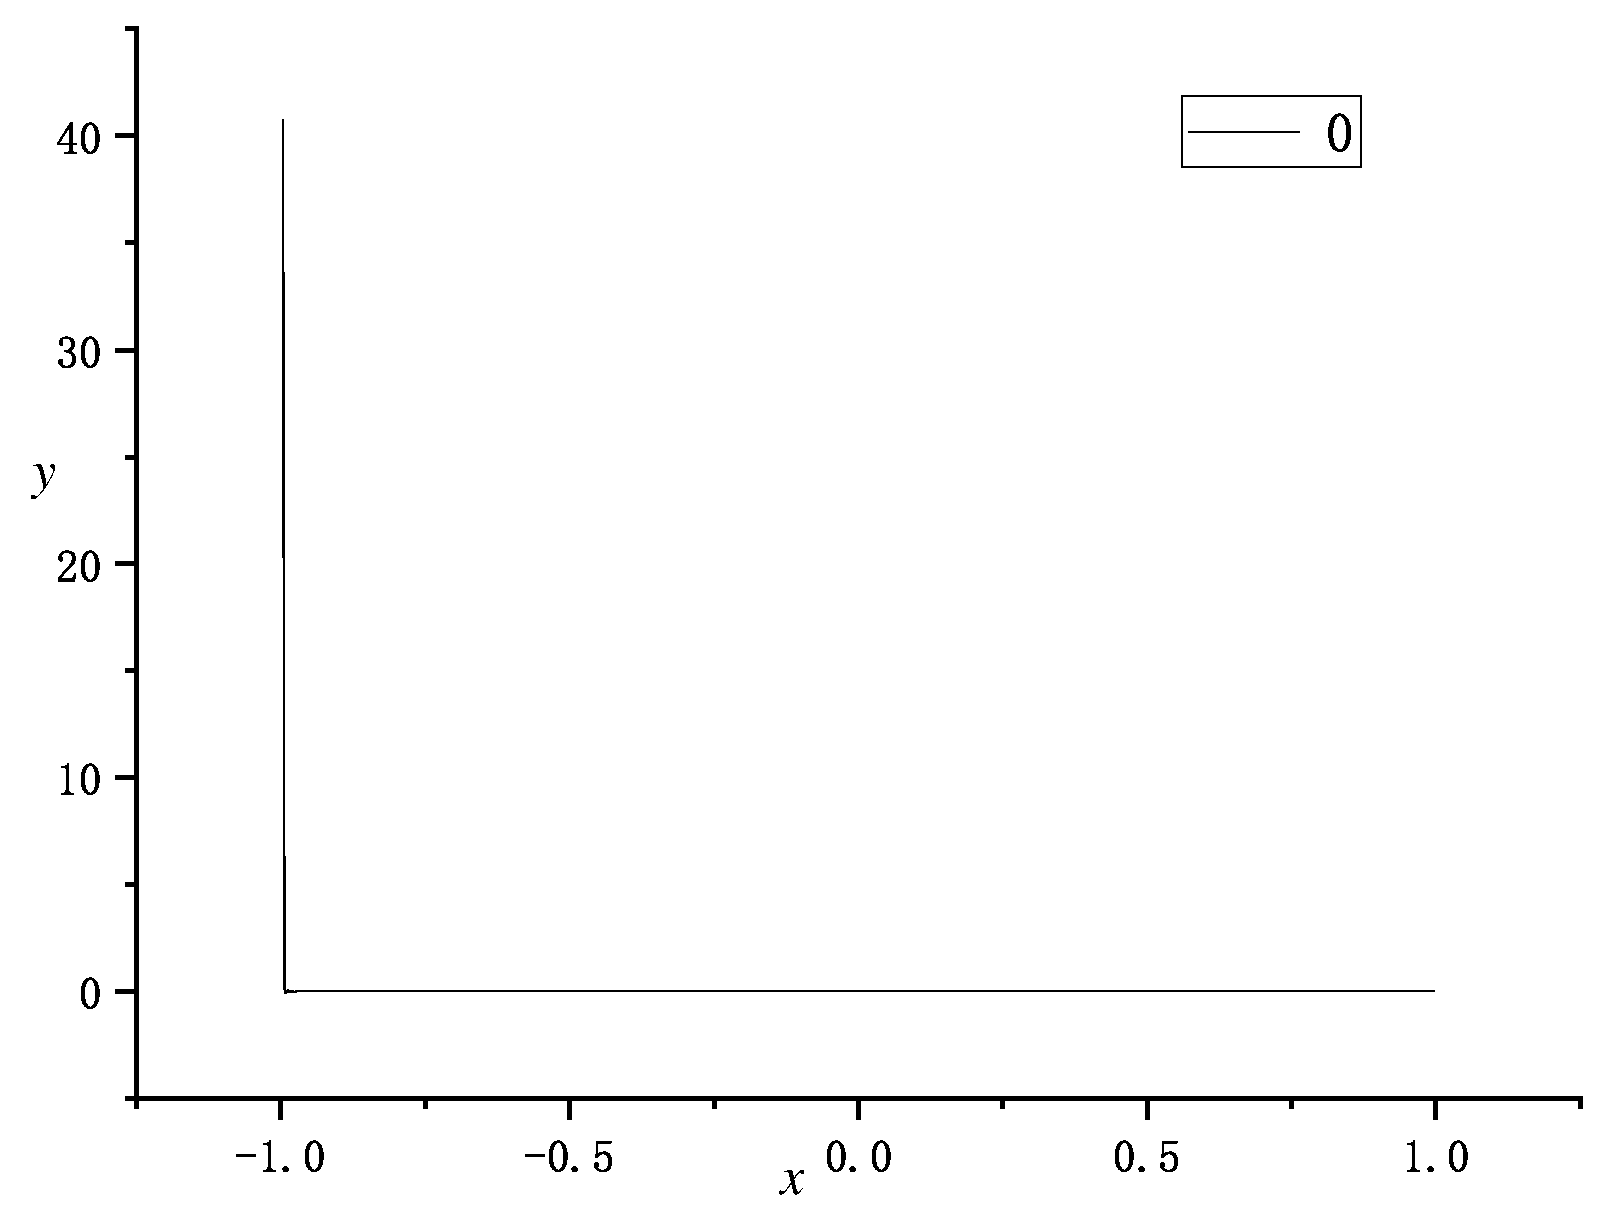
\includegraphics[width=5.5cm]{9.pdf}}\quad
                \subfigure[Chebyshev(128), $j=64$]{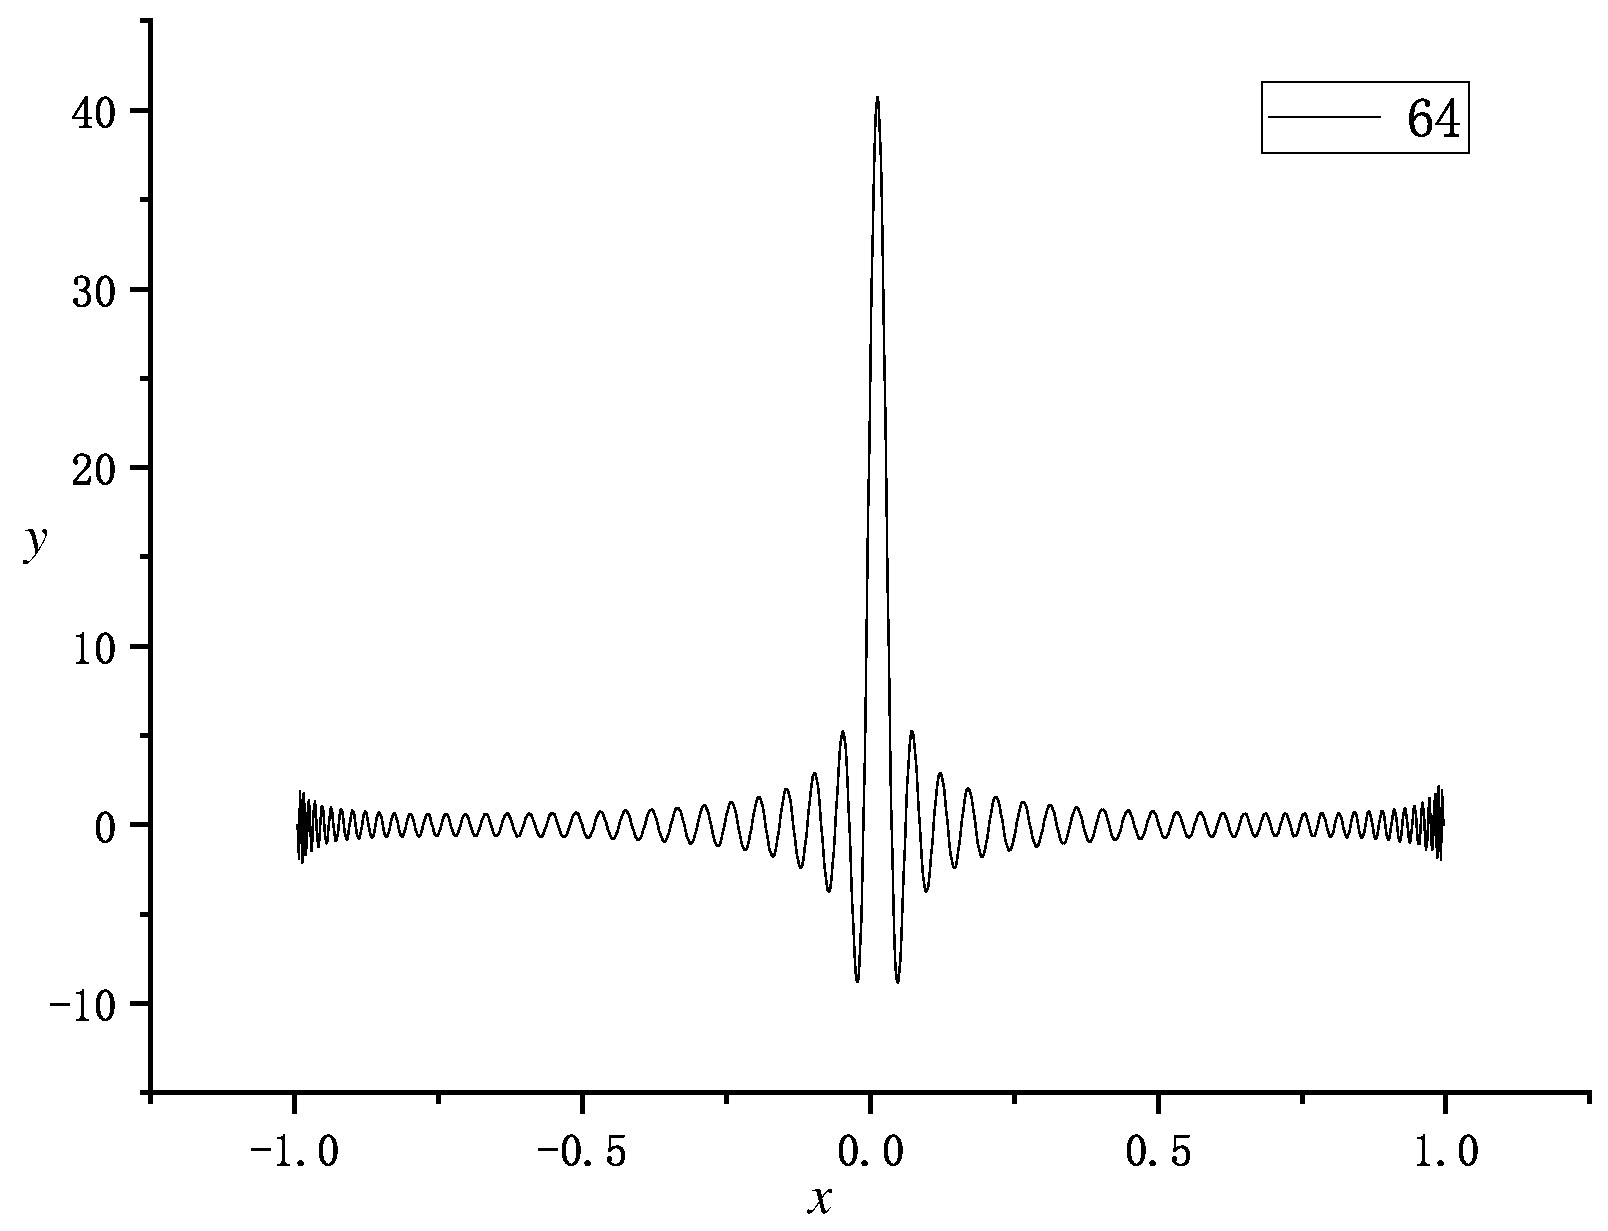
\includegraphics[width=5.5cm]{10.pdf}}\quad
            \end{figure}
    \bibliographystyle{unsrt}
    \bibliography{citation}
\end{document}